\subsection{Mesh > Smooth (Laplacian)}
\label{subsection:samplePoints}
\index{echantillonner@�chantillonner!des points sur un maillage}

Cette fonction lisse un maillage par approche de type Laplacien (voir figure~\ref{fig:laplacianSmooth}). Attention, ce type d'approche ne conserve pas la volume du maillage. De plus, les sommets du maillage sont d�plac�s.\\

\begin{figure}[!h]
\begin{center}
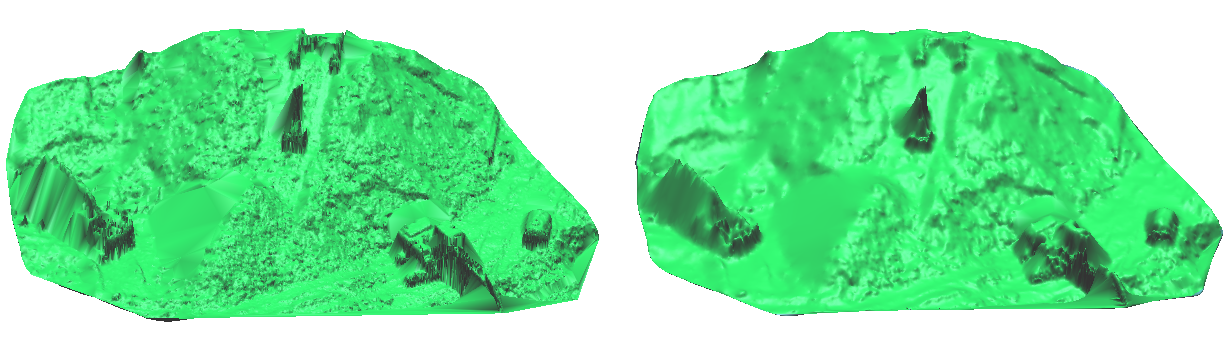
\includegraphics[width=0.9\textwidth]{Partie3_Fonctions/meshLaplacianSmooth.png}
\caption{\label{fig:laplacianSmooth}Maillage avant (� gauche) et apr�s (� droite) lissage de type \textit{Laplacien}}
\end{center}
\end{figure}

\par
Avant d'appliquer cette fonction, CloudCompare demande � l'utilisateur de d�finir deux param�tres :
\begin{itemize}
\item le nombre d'it�rations : plus les it�rations sont nombreuses, plus le lissage est fort... et plus la m�thode est longue.
\item la force du lissage � chaque it�ration : plus celle-ci est �lev�e, et plus le lissage est fort (ce qui peut permettre de diminuer le nombre d'it�rations - voir ci-dessus) mais plus les risques de probl�mes topologiques sont �lev�s.\\
\end{itemize}
